\chapter{Hyperspectral}

%TODO translate using  Hyperspectral_tr.txt
A hyperspectral image contains a collection of spectral pixels or
equivalently, a collection of spectral bands.

\begin{figure}[h]
  \centering
  \includegraphics[width=0.7\textwidth]{Cube_HPX.eps}
  \itkcaption[Hyperspectral cube]{Illustration of an hyperspectral cube, spectral pixel and a spectral layer.}
  \label{fig:cube}
\end{figure}

An hyperspectral system \ref{fig:cube} acquired
radiance, each pixel contains fine spectral information
fine that depends of:

\begin{itemize}
\item{Spectrum of the light source (in practice, the
sun) and atmospheric disturbances.}
\item{Spectral responses
of different materials in the overlap zone and of the nature of the mixture.}
\end{itemize}

Preliminary treatments allow to perform 
atmospheric correction for estimating a reflectance cube
spectral by subtraction of information extrinsic of the
scene (see also \ref{secAtmosphericCorrections}).
 
\section{Unmixing}

\subsection{Linear mixing model}

Reflectance information depends only of the materials spectral responses in the scene. When the mixture between
materials is macroscopic, the linear mixing model of spectra
is generally admitted. In this case, the image typically looks like this:

\begin{figure}[h]
  \centering
  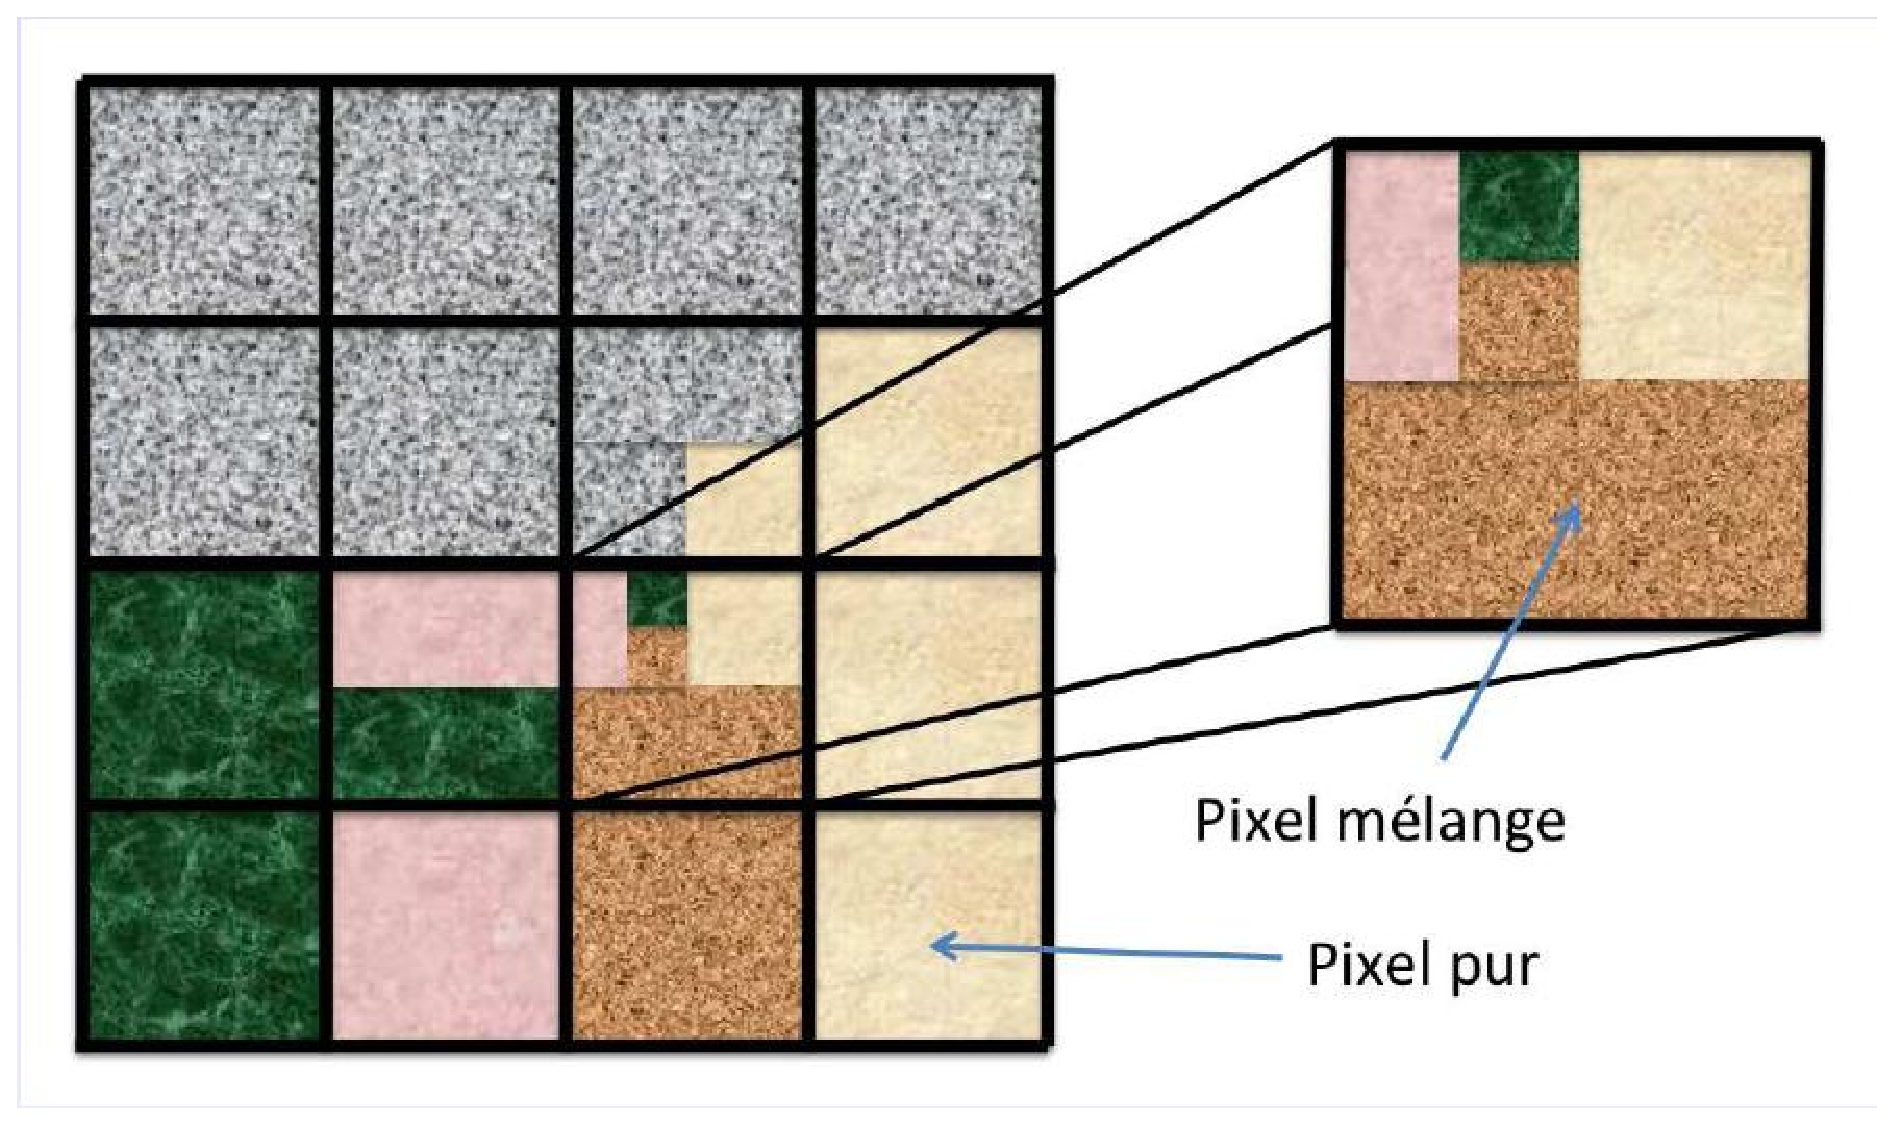
\includegraphics[width=0.7\textwidth]{Linear_Unmixing_HPX.eps}
  \itkcaption[Linear mixing model]{Zone which verify the LM model.}
  \label{fig:linear_unmixing}
\end{figure}

We notice \ref{fig:linear_unmixing} the
presence of pure pixels, and pixel-blending. The LMM acknowledges that
reflectance spectrum associated with each pixel is a linear combination of pure materials in the recovery area, commonly known as ``''endmembers. This is illustrated in \ref{fig:decomp_mml}

\begin{figure}[h]
  \centering
  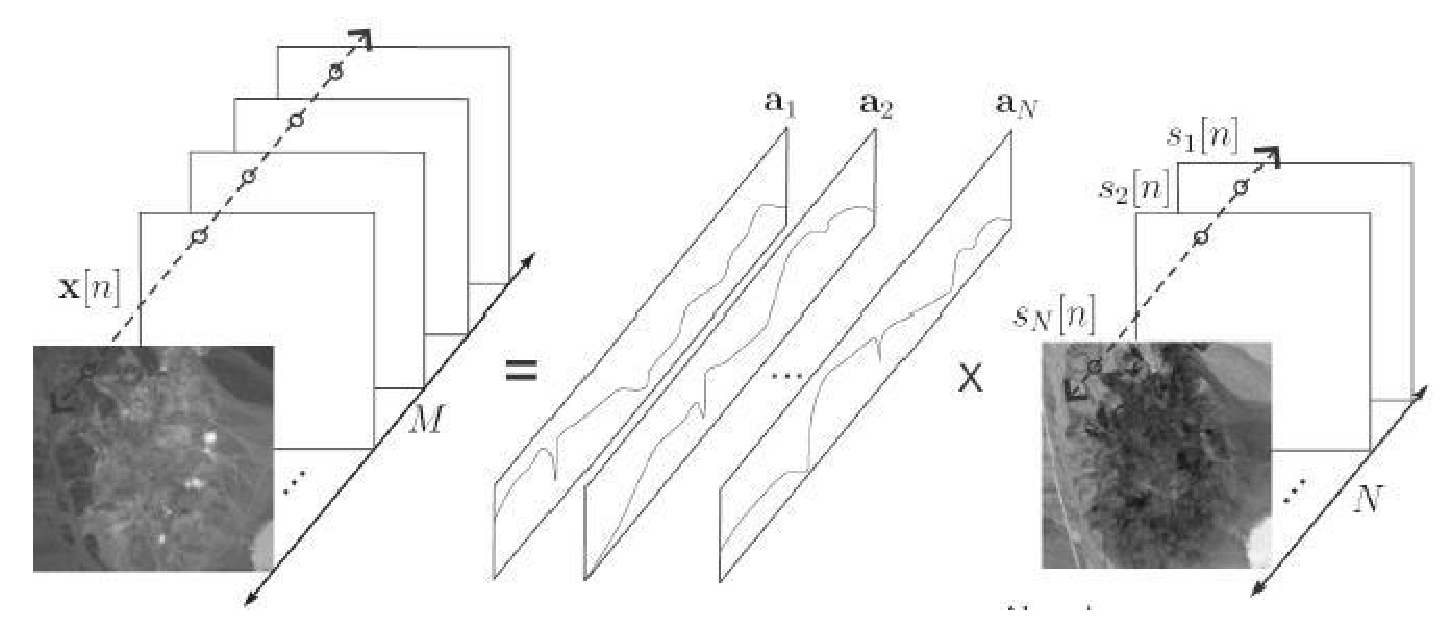
\includegraphics[width=0.7\textwidth]{Decomposition_MML_HPX.eps}
  \itkcaption[Decomposition of the LMM]{Decomposition of a hyperspectral cube according to the LMM.}
  \label{fig:decomp_mml}
\end{figure}
The `` left'' term represents the different spectral bands of
data cube. The `` right'' term represents a `` product''
between the reflectance spectra of endmembers and their repective abundances. Abundance band of endmembers is
image grayscale between $0$ and $1$. The pixel i of the
abundance band of endmember j is $s_ {ji}$. This value is the
abundance of endmember j in the pixel i. Under certain conditions
[Huck2009], this value can be interpreted as the ratio
surface of the material in the overlap zone (\ref{fig:linear_unmixing}). In
practice, one can reasonably expect that: 

\begin{itemize}
\item{a limit number
of pure materials compose the scene.}
\item{the scene contains pure pixels if the spatial resolution is sufficient and
do not necessarily contains them otherwise.}
\end{itemize}

Many techniques of unmixing in hyperspectral image analysis
are based on geometric approach where each pixel is seen as a spectral
vector of L (number of spectral bands). The
spectral bands can then be written as vectors.

\begin{figure}[h]
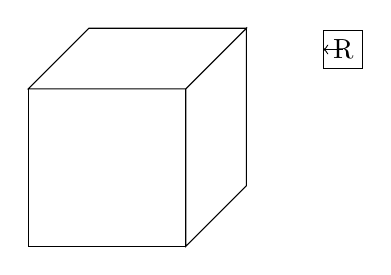
\begin{tikzpicture}
\pgfmathsetmacro{\cubex}{2}
\pgfmathsetmacro{\cubey}{2}
\pgfmathsetmacro{\cubez}{2}
\draw[black,fill=white] (0,0,0) -- ++(-\cubex,0,0) -- ++(0,-\cubey,0) -- ++(\cubex,0,0) -- cycle;
\draw[black,fill=white] (0,0,0) -- ++(0,0,-\cubez) -- ++(0,-\cubey,0) -- ++(0,0,\cubez) -- cycle;
\draw[black,fill=white] (0,0,0) -- ++(-\cubex,0,0) -- ++(0,0,-\cubez) -- ++(\cubex,0,0) -- cycle;
\node[draw] (R) at (2,0.5) {R};
\draw[->] (2,0.5) -- (R.west);
\end{tikzpicture}
\itkcaption[Hyperspectral cube vectorization]{``Vectorization'' of hyperspectral cube. The spectral pixels
are stored in the columns of the matrix R and, in
equivalently, the spectral bands are assigned to the lines of R.}
\label{fig:mml}
\end{figure}
%% Figure 5: "Vectorisation" du cube hyperspectral. Les pixels spectraux
%% sont ranges dans les colonnes de la matrice R et, de maniere
%% equivalente, les bandes spectrales sont rangees dans les lignes de R.

By deduction of \ref{fig:decomp_mml} et de \ref{fig:mml}, the LMM needs to decompose R as: 
\begin{center}
$R= A.S + N = X + N$
\end{center}

J is the number of endmembers and the number of spectral pixels I:
 
\begin{itemize}
\item{Les J colonnes de la matrice A contiennent les spectres de endmembers.}
\item{Les J lignes de la matrice S contiennent les cartes d'abondances
vectorisees;nous appelons vecteurs d'abondances les colonnes de la
matrice S.}
\item{La matrice N, de dimensions $LxI$, est une matrice de bruit
additif.}
\end{itemize}

   

Le probleme du demixage consiste a estimer les matrices A et S a
partir de R ou eventuellement de \"X, une estimation de la matrice signal
debruite.

Plusieurs contraintes physiques peuvent être prises en
compte pour permettre la resolution de ce probleme: 
\begin{itemize}
\item{C1: positivite
des spectres de reflectance (matrice A non-negative).}
\item{C2: positivite
des abondances (matrice S non-negative).}
\item{C3: additivite des
abondances (la somme des coefficients de chaque colonne de la matrice
S vaut 1).}
\item{L'independance algebrique entre les ``vecteurs spectraux''
associes au endmembers et la linearite des melanges de spectres, d'ou
decoule la propriete du simplexe decrite au paragraphe suivant.}
\end{itemize}

\subsection{Simplex}  
Les algorithmes recents de demixage s'appuient sur la ``propriete du
simplexe''. Dans un espace vectoriel de dimension $J-1$, on peut
associer a J vecteurs algebriquement independants J points definissant
les sommets d'un J-simplexe \ref{fig:simplex}.

\begin{figure}[h]
  \centering
  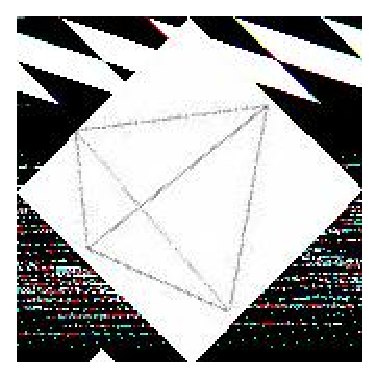
\includegraphics[width=0.7\textwidth]{Simplex_HPX.eps}
  \itkcaption[Simplex]{Illustration d'un 2-simplexe, d'un 3-simplexe et d'un
4-simplexe.}
  \label{fig:simplex}
\end{figure}

Un cube hyperspectral de L bandes, base sur J endmembers,
peut etre confine dans un sous-espace-affine de dimension $J-1$.  
Un sous espace pertinent, au sens du rapport signal-a-bruit, est
generalement obtenu par Analyse en Composantes Principales (ACP). En
pratique, les $J-1$ vecteurs propres associes au plus fortes valeurs
propres forment les colonnes d'une matrice de projection V de
dimension $(Lx(J-1))$. Les donnees reduites Z, de dimensions
$((J-1)xI)$, sont obtenues par l'operation:
$Z=V^{T}(\tilde{R})$

ou chaque colonne de $\tilde{R}$ est vue soustraire le spectre moyen,
generalement estime au sens du maximum de vraisemblance. Dans le
sous-espace porteur des vecteurs-colonnes de Z, les spectres de
endmembers sont donc associes au sommet d'un simplexe. Si le bruit est
negligeable, ce simplexe circonscrit les donnees reduites.

Cette propriete met en evidence le fait que les endmembers
recherches sont les sommets d'un simplexe qui circonscrit les
donnees. Cependant, une infinite de simplexes differents peuvent
circonscrire un meme jeu de donnees. En fait, le probleme du demixage
n'a generalement pas de solution unique. Cette degenerescence peut
aussi etre mise en evidence par le formalisme de la factorisation en
matrices non-negatives (voir Huck2010a), qui sera aborde un peu plus
loin. Il convient donc de choisir la solution physiquement la plus
pertinente. Toutes les techniques de demixage basees sur cette
propriete du simplexe admettent que la solution la plus pertinente est
definie par le simplexe admissible de volume minimal, ou la notion de
volume est generalisee a toutes les dimensions finies (eventuellement
differentes de 3).  

\subsection{Selection d'algorithmes et etat de l'art} 
Les algorithmes de demixage lineaire les plus recents exploitent
generalement la propriete du simplexe. Il est possible de les classer
en plusieurs familles:
\subsubsection{Famille 1} 
Une premiere famille d'algorithmes
de demixage est basee sur la recherche des endmembers ``parmi'' les
donnees. Cela signifie qu'un pixel pur au minimum doit etre associe a
chaque endmembers. Si cette hypothese n'est pas verifiee, cela
produira une erreur d'estimation sur les spectres de
endmembers. L'avantage historique de ces algorithmes est leur faible
complexite algorithmique. Les trois plus connus sont PPI (Pixel Purity
Index), NFINDER et VCA (Vertex Component Analysis)
[Nascimento2005]. Outre son succes reconnu par la communaute et sa
complexite algorithmique tres competitive, l'estimation des spectres
de endmembers est non biaisee en l'absence de bruit (et lorsque il y a
des pixels purs).

\paragraph{VCA} 
Note: L'algorithme VCA est systematiquement
utilise pour initialiser les differents algorithmes etudies (sauf
MVES, base sur une autre initialisation).

Elements importants sur le fonctionnement de VCA: 
\begin{itemize}
\item {L'algorithme VCA
est base sur des projections iteratives des donnees orthogonales au
sous-espace porte par les endmembers deja estimes.}
\item {Biaise lorsque le
degre de purete est inferieur a 1.}

\end{itemize}  

\subsubsection{Famille 2} 
Une deuxieme famille est composee d'algorithmes recherchant le
simplexe de volume minimal circonscrivant les donnees. La phase
d'initialisation consiste a determiner un simplexe initial quelconque
circonscrivant les donnees. Puis, un schema d'optimisation numerique
permet de minimiser une fonctionnelle, fonction croissante du volume
generalise, lui-meme dependant des endmembers estimes a l'iteration
courante. L'optimisation est contrainte par le fait que les donnees
doivent restees inscrites dans le simplexe et eventuellement par les
contraintes C1, C2 et C3.

Les algorithmes existant sont : 
\begin{itemize}
\item {MVSA (Minimum Volume Simplexe
Analysis) [Li2008].}
\item { MVES (Minimum Volume Encosing Simplex)
[Chan2009].}
\item {SISAL (Simplex Identification via Split Augmented
Lagrangian) [Dias2009].}
\end{itemize}  
  
Les differences principales entre les algorithmes consideres
concernent: 
\begin{itemize}
\item {Le schema d'optimisation numerique.}
\item {La maniere dont les
contraintes sont prise en compte.}

\end{itemize}  

 
Ces points impactent la complexite algorithmique et la precision
d'estimation. 
 
\paragraph{MVSA aLi2008]} 
Elements importants sur le fonctionnement de MVSA: 
\begin{itemize}
\item {Initialisation par VCA.}
\item {Tous les pixels spectraux inclus dans le simplexe estime
  (approximativement) par VCA n'impactant pas la contrainte
  d'inscription des donnees dans le simplexe recherche, ils sont
  simplement supprimes des donnees utilisees dans la phase de
  minimisation du simplexe afin de reduire la complexite
  algorithmique.}
\item {La technique d'optimisation tres evoluee est de type
  programmation quadratique sequentielle (Sequencial Quadratic
  Programming - SQP) et plus precisement a la categorie
  ``quasi-Newton'' sous contrainte.}
\end{itemize} 

\paragraph{MVES [Chan2009]}
 Elements importants sur le fonctionnement de MVES: 
\begin{itemize}
\item {Initialisation par une
  methode iterative (Programmation Lineaire LP pour Linear
  Programming) non-triviale et differente de VCA.}
\item {Resolution du
  probleme par LP.}
\end{itemize} 
 

\paragraph{SISAL [Dias2009]}
Elements importants sur le fonctionnement de SISAL: 
\begin{itemize}
\item {Initialisation
par VCA.}
\item {Selection des pixels spectraux analogue a MVSA pour reduire
la complexite algorithmique.}
\item {Technique d'optimisation tres evoluee
cumulant plusieurs particularites.}
\begin{itemize}
\item {Decomposition du probleme
non-convexe en serie de problemes convexes.}
\item {Developpement d'une
methode specifique de separation de variables permettant de considerer
un lagrangien augmente avec de bonnes proprietes de calcul.}
\end{itemize}
\end{itemize} 

\subsubsection{Famille 3}
Il s'agit d'algorithmes de Factorisation en matrices non-negatives
(NMF pour Non-negative Matrix Factorization). L'objectif de cette
branche des mathematiques appliquees est de factoriser une matrice
non-negative, X dans notre cas, en produit de matrices
non-negatives:AS par minimisation d'une distance entre X et AS et
avec une regularisation adaptee, afin de lever la degenerescence de
maniere adaptee au probleme physique associe au demixage.
\paragraph{MDMD-NMF [Huck2010b]} 
Elements importants sur le fonctionnement de MDMD-NMF:
\begin{itemize}
\item {Initialisation par VCA.}
\item {Minimisation de la norme de la norme de
Frobenius avec une regularisation spectrale et une regularisation
``spatiale'' (sur la matrice d'abondances).}
\begin{itemize}
\item {Minimum spectral
Dispersion: la regularisation spectrale encourage la variance des
coefficients d'un spectre de endmembers a etre faible.}
\item {Maximum spatial Dispersion: la regularisation spatiale
  encourage les vecteurs d'abondances a occuper toute la partie
  admissible (plus d'information dans [Huck2009]). Cette action
  presente une certaine analogie a la contrainte de volume minimum.}
\end{itemize}
\end{itemize}
 
 
  

\subsubsection{Remarques complementaires}
Les algorithmes des familles 1 et 2 estiment les spectres de
endmembers ``seulement''. L'estimation des cartes d'abondances a lieu
a posteriori et requiert l'application d'un algorithme de type Fully
Constrained Least Square (FCLS) [Heinz2001]. MVES inclut un algorithme
specifique d'estimation des abondances, que nous avons utilise dans
nos simulations (pour MVES seulement).  
Le demixage est un probleme generalement non convexe, ce
qui explique l'importance de l'initialisation des algorithmes.
Recapitulatif de la prise en compte des differentes contraintes
physiques:


\begin{center}
   \begin{tabular}{ l | l | l | l | l | l }
     \hline
     & VCA & MVSA & MVES & SISAL & MDMD \\ \hline
     C1 $(A>0)$ & muette & Muette & Muette & Muette & Dure \\ \hline
     C2 $(S>0)$ & muette & Dure & Dure & Souple & Dure \\ \hline
     C3 (additivite) & Muette (via FCLS) & Dure & Dure & Dure & Souple \\ \hline
     simplexe & Endmembers \newline parmi les donnees & Circonscrit \newline aux donnees & 
     Circonscrit \newline aux donnees & Circonscrit \newline aux donnees &
     Indirecte par la \newline regularisation ``spatiale'' \\ \hline
   \end{tabular}
 \end{center}

\section{Dimensionality reduction}

\section{Anomaly detection}
Une anomalie dans une scene est, par definition, un element qu'on ne
s'attend pas a y trouver. L'element anormal est donc de nature
differente de son environnement et sa presence est minoritaire dans la
scene. Typiquement, un vehicule dans en milieu naturel, un rocher dans
champ, une cabane en bois dans une foret suffisamment clairsemee sont
autant d'anomalies que l'on peut souhaiter detecter a l'aide
d'imagerie hyperspectrale. Cela suppose que la reponse spectrale de
l'anomalie puisse etre discriminee de la reponse spectrale du
``fouilli-du-fond'' (background clutter). Cela suppose egalement que
les pixels associes aux anomalies, les pixels anormaux, sont
suffisamment rares et/ou ponctuels pour pouvoir etre consideres comme
tels. Ces proprietes peuvent etre vues comme des hypotheses spectrales
et spatiales sur lesquelles s'appuient les techniques de detection
d'anomalies dans les images hyperspectrales.

Nous rappelons que la litterature relative a l'imagerie hyperspectrale
distingue generalement la detection de cibles et la detection
d'anomalies:

\begin{itemize}
\item {On parle de detection de cibles lorsque la reponse
spectrale de l'element recherche est utilisee en entree de
l'algorithme de detection. Il s'agit d'information a priori qui
permet, en theorie, de construire des algorithmes a tres fort pouvoir
de detection, tels que l'Adaptive Matched Filter (AMF) ou l'Adaptive
Cosine/Coherence Estimator (ACE),pour n'en citer que deux. Neanmoins,
la connaissance suffisamment fine du spectre recherche est une
information difficile a detenir en pratique, ce qui conduit bien
souvent a l'utilisation d'algorithmes de detection d'anomalies.}
\item {On parle de detection d'anomalies lorsque le spectre de
  l'element anormal n'est pas requis par l'algorithme de
  detection. Pour cette raison, on associe souvent le terme de
  ``detection non supervisee''. Neanmoins, les algorithmes dependent
  generalement de ``parametres de structure''. Par exemple, dans le
  cas de la detection dans une fenetre glissante, le juste choix des
  dimensions repose sur une connaissance a priori de la taille des
  anomalies recherchees. Cette partie de l'etude se concentre sur la
  comparaison d'algorithmes de detection d'anomalies.}
\end{itemize}
    
\begin{figure}[h]
  \centering
  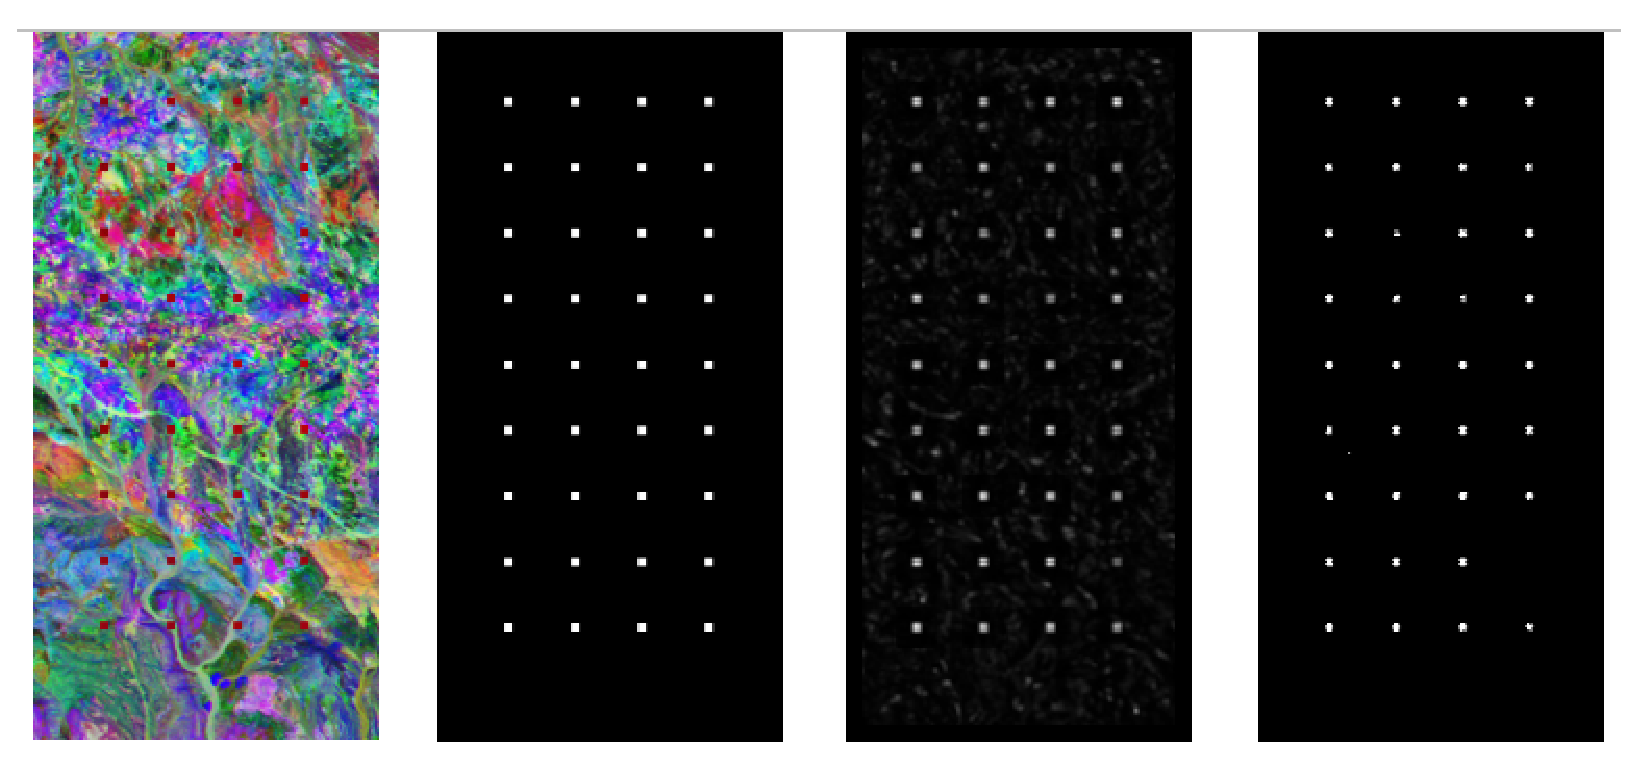
\includegraphics[width=0.7\textwidth]{Anomaly_HYP.eps}
  \itkcaption[Notion sur la detection]{Notions sur la detection: masque de verite terrain, carte de detection, masque de detection.}
  \label{fig:anomaly_hyp}
\end{figure}
In \ref{fig:anomaly_hyp}, nous introduisons d'ores et deja quelques notions
qui seront utiles par la suite. Les algorithmes de detection
d'anomalies ont comme entree une image et estiment une carte de
detection faisant office d'outil d'aide a la prise de decision. Un
seuillage adapte permet d'obtenir un masque de detection estime, que
l'on espere le plus ressemblant possible au masque de verite terrain,
inconnu en pratique. Ce masque estime a la vocation d'un outil de
prises automatiques de decisions.

Deux approches dominent l'etat de l'art sur la detection d'anomalies
dans les images hyperspectrales. Il s'agit des methodes par Poursuite
de Projection (PP) et les methodes basees sur une modelisation
probabiliste de la classe fond et eventuellement de la classe cible
avec test d'hypotheses statistiques.
La PP consiste a projeter lineairement les pixels spectraux sur des
vecteurs wi qui optimise un critere sensible a la presence d'anomalies
(ex: kurtosis). On obtient une serie de cartes de projections ou les
anomalies contrastent tres fortement avec le fond. Mais l'estimation
automatique d'une carte de detection presente des difficultes
majeures, notamment:
\begin{itemize} 
\item Combien de projecteurs doit-on estimer?  
\item Quel(s) projecteur(s) choisir?  
\item Comment gerer un fond inhomogene?  
\item Les performances de detection varient avec les dimensions spatiales de l'image (nombre d'echantillons) 
\item Ces algorithmes ont generalement une structure peu parallelisable
\item Ces algorithmes ne sont generalement pas ``a taux de fausse alarme constant''.
\end{itemize}

Les algorithmes selectionnes sont RX (presente en premiere version
dans [Reed1990] et GMRF [Schweizer2001] et leurs specificites
respectives seront presentees plus loin. Ils sont bases sur les
notions de modeles probabilistes, test d'hypotheses statistiques et
fenetre glissante.  Ce type d'approche consiste a repondre a la
question: ``Le pixel (ou ensemble de pixels voisins) teste
ressemble-t-il au pixels du fond?'' par une demarche de test
statistique. De maniere plus exhaustive, cette demarche necessite:
\begin{itemize} 
\item Un modele pour la classe ``fond'' 
\item Le choix d'un test statistique 
\item Eventuellement, un modele pour la classe ``anomalie''
\item Des estimateurs pour les differents parametres inconnus a priori
\item Des hypotheses d'homogeneite permettant un compromis satisfaisant entre: 
\begin{itemize} 
\item Le nombre d'echantillons en regard du nombre de parametres a
  estimer 
\item L'homogeneite, notamment du fond 
\item La complexite algorithmique (quoique les algorithmes consideres sont
hautement parallelisables)
\end{itemize} 
\end{itemize} 
Le principe de fonctionnement de RX et GLRT peut etre resume par les
Figure 27  et Figure 28.
(TODO do block diagramme using tikz)

Une premiere etape facultative (spontanement consideree dans le cadre
de cette etude) consiste a reduire la dimension spectrale des donnees
tout en conservant l'information liee aux anomalies. Puis, les pixels
spectraux sont testes a tour de rôle (tache parallelisable). Le pixel
teste se voit attribuer une fenetre glissante (voir Figure 28). Cette
fenetre comprend deux sous fenetres, centrees sur le pixel teste, de
dimensions respectives L et LL, avec $L < LL$. 
\begin{itemize}
\item Les pixels appartenant a la couronne ainsi formee appartiennent
  a la classe ``fond local''. Les parametres statistiques du fond,
  requis par les tests statistiques, sont estimes a partir de ces
  pixels spectraux. L'une des difficultes consiste a trouver un
  compromis sur l'epaisseur de la couronne (et donc le nombre
  d'echantillons statistiques) sachant que: 
\begin{itemize}
\item Si la couronne est trop epaisse, le fond local n'est plus
  suffisamment homogene 
\item Si le nombre d'echantillons est trop faible, la precision de
  l'estimation statistique des parametres du modele du fond est trop
  faible
\end{itemize}  
\item Les pixels de la partie centrale de la fenetre glissante
  appartiennent a la classe ``inconnue''. Si le pixel teste (pixel
  central) est un pixel anormal, il est possible que ses voisins
  soient aussi des pixels anormaux, d'ou l'interet de ne pas choisir
  une valeur de L trop faible si l'on sait que les anomalies
  recherchees peuvent etre reparties sur plusieurs pixels.
\end{itemize}  
Une fois l'ensemble des
parametres estimes, un test statistique est effectue et affecte une
valeur $\Lambda(i)$ au pixel teste i. Une carte de detection est ainsi
constituee.

Figure 28: Principe de la fenetre glissante et definitions des
parametres L et LL de la fenetre glissante.  Les algorithmes RX et
GMRF, consideres dans presentes dans les sections suivantes.
(TODO  block diagram for windowing using tikz)

\subsection{Local RX}
